\section{Introduction}
\label{sec:intro}

\begin{figure}[t]
\begin{center}
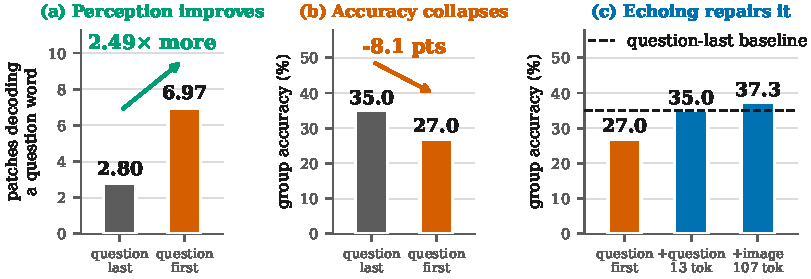
\includegraphics{figs/fig_teaser.pdf}
\end{center}
\caption{The question-first paradox and its repair, Qwen3-VL-8B.
\textbf{(a)} Question-first makes $2.49\times$ more image patches decode a
question content word (160 NaturalBench candidates), so the question reaches the
image. \textbf{(b)} It still loses $8.1$ points of group accuracy
($p = 1.3\times10^{-12}$). \textbf{(c)} Echoing the question after the image
repairs it for $13$ tokens; an $\tfrac{1}{8}$-resolution image echo beats the
baseline for $107$.}
\label{fig:teaser}
\end{figure}

Ask a vision-language model a question about an image and you must decide, often
without thinking about it, whether the question goes before the image or after
it. The information content is identical either way. Under causal attention,
putting the question first is the option that lets every image token see it,
which is what a reader would want when told to look for something specific.

It makes the model worse. Moving the question before the image costs Qwen3-VL-8B
$8.1$ points of NaturalBench group accuracy
($p = 1.3\times10^{-12}$), $9.5$ points on Winoground, and $18.0$ points on
CV-Bench, with an average loss of $7.0$ points across 13 benchmarks. The same
reversal holds for Qwen2.5-VL-7B, InternVL3-8B and LLaVA-1.5, which reaches
exactly zero group accuracy when the question comes first.

The obvious explanation is that question-first prompting damages perception, and
it is wrong. Reading image patches with a logit lens, question-first makes
$2.49\times$ more patches decode a content word from the question than
question-last does ($6.975$ against $2.800$ per image), and the question
measurably rewrites those tokens, moving them nearly twice as far from an
image-only forward pass as the system message alone. The ordering that looks most
like it has found the answer is the one that gets it wrong. We call this the
question-first paradox.

We locate the failure in read-out rather than perception. At the layer where the
answer position attends most strongly to the question, question-first sends
$2.19\times$ less attention mass there and $2.51\times$ more to the image. The
two orderings are indistinguishable at chance through layer 25 of 36 and then
diverge to $P(\text{correct})$ of $0.0986$ against $0.8747$. Severing attention
edges shows the dependence is causal and doubly dissociated: cutting the
answer-to-question path costs question-last $5.6$ points and question-first
nothing, while cutting the answer-to-image path costs question-first $9.6$ points
and question-last nothing.

That diagnosis prescribes the prompt. If the answer position cannot read the
question, put something after the image that it can read. Repeating the question
(\stit{}) costs $13$ tokens, recovers $78\%$ of the deficit, and provably cannot
change perception: the image tokens stay identical to five decimals. Repeating
the image (\sitit{}) recovers the deficit entirely and adds $1.18$ points over
question-last across 13 benchmarks. Neither repair supplies new information. A
reversed echo works as well as a correct one, and an eighth-resolution echo
matches a full one at $3\%$ of the added tokens. A reflective prompt optimizer,
given the same budget, gains only under the ordering the diagnosis says has
headroom and never reaches the question-last baseline it competes with.
